\chapter{Analyser}\label{Analyser}

\section{Brugerundersøgelse}
Der er foretaget to slags brugerundersøgelser: en spørgeskemaundersøgelse med potentielle patienter og to interviews med henholdsvis en radiolog og en radiograf. Dette er medtaget for at belyse, hvordan en automatiseret ultralydsscanner til screening for brystkræft vil modtages af patienter og personale. 

\subsection{Spørgeskemaundersøgelse}
Undersøgelsen, bestående af et kvalitativt spørgeskema med tre spørgsmål samt spørgsmål om aldersgruppe og køn, er lavet for at undersøge potentielle patienters meninger om at blive undersøgt af en automatiseret robot. Der blev spurgt om tanker angående scanning af en automatisceret  robotarm fremfor en læge, samt hvilke problemstillinger og fordele respondenterne ser ved en automatiseret ultralydsscanner. Undersøgelsen er derefter kvantificeret på baggrund af respondenternes svar. 

Der var i alt 72 respondenter på spørgeskemaet, hvor størstedelen, 87,5\%, af respondenterne var positive for at blive scannet af robotarmen, hvis kvaliteten og sikkerhed er på højde med, hvad den er, når en læge foretager en ultralydsscanningen. De sidste 12,5\% som var negative for automatisk scanning med en robotarmen, frygter, at robotarmen vil lave fejl, det bliver upersonligt, og at det vil give en fornemmelse af, at lægen har berøringsangst for patienterne. 
De problemstillinger respondenterne ser ved automatiserede ultralydsscanninger var, at robottens følsomhed mangler, og det måske kan gøre undersøgelsen ubehagelig og utryg for patienten. Samtidig nævner flere bekymringer for robottens evne til at scanne forskellige kropstyper. Fordelene, som respondenterne så ved automatiserede ultralydsscanninger var, at robotten måske kan give økonomisk mening med kortere ventetider og spare tid og dermed frigøre ressourcer i form af personale til andre opgaver. Flere af respondenter mente, at en robotarm kan reproducere scanningerne og er derfor ikke afhængig af, hvor god lægen er. Den yngre del af respondenterne nævner ergonomiske fordele for lægen, mindre blufærdighed og langdistance-undersøgelser, som andre fordele. 

Spørgeskemaundersøgelsen blev lavet før projektet var færdigdefineret, og derfor falder den lidt ved siden af projektet. Den er dog stadig medtaget i projektet, fordi den kan give en indikation af, hvordan og hvad der skal til før patienter vil tage imod Automatisk Ultralydsscanner. 

Se bilag \ref{Sporgeskemaundersogelse} Spørgeskemaundersøgelse, for hele analysen. 

\subsection{Interview med radiograf} 
Aarhus Universitetshospital, Tage-Hansens Gade blev kontaktet til inspiration og belysning af den daglige praksis på en røntgen- og skanningsafdeling, samt undersøgelse af sundhedsfagliges meninger om Automatisk Ultralydsscanner. Radiograf Tine Bisgaard indvilgede i at vise rundt på afdelingen samt svare på spørgsmål om afdelingens dagligdag. På daværende tidspunkt var Automatisk Ultralydsscanner ikke afgrænset til at kunne indgå i som supplement til mammografi i screeningspakken. 

Tine Bisgaard vurderede mammografi af begge bryster til at tage 5 minutter, mens en ultralydsscanning blev vurderet til at tage omkring 10 minutter, afhængigt af radiologens rutine. Tine Bisgaard mente ikke, at det vil være et problem at benytte en Automatisk Ultralydsscanner til at udføre scanninger, hvis man blot informerer patienterne. Hun ser dog en ulempe ved at lade en radiograf lave scanningerne idet, patienten ikke kan få svar med det samme, hvilket de normalt får når en radiolog udfører ultralydsscanningen. Tine Bisgaard nævnte yderligere en ulempe, hun frygter at det vil tage længere tid at foretage scanningen og derefter få en radiolog til at vurdere billederne.

Fordelene, Tine Bisgaard ser ved en Automatisk Ultralydsscanner er, at man på afdelingerne er nødt til at tænke i nye baner ift. manglen på radiologer i Danmark. Derfor mener hun, at det vil være smart, hvis radiograferne kunne udføre en del af arbejdet med ultralyd for at spare tid og penge.

På baggrund af dette besøg blev der udspecificeret nogle af kravene til Automatisk Ultralydsscanner.

Se bilag \ref{Tine} Interview med afdelingsradiograf Tine Bisgaard, for hele interviewet. 

\subsection{Interview med radiolog}
Der blev foretaget et telefonisk interview og efterfølgende et opfølgende møde med radiolog og ultralydsekspert, Lars Bolvig. Interviewet blev lavet for at undersøge proceduren ved ultralydsscanninger af brystet. Der var på forhånd defineret nogle spørgsmål angående lokalisering af knuder, hastigheder og tiden en læge typisk vil bruge på en ultralydsscanning af brystet og lokalisering af knuder. Ifølge Lars Bolvig vil en læge kunne lokalisere en knude i brystet på 2-3 minutter, mens hastigheden, der scannes med, er meget operatørafhængig. Lars Bolvigs forslag til hvor det vil give mening at implementere Automatisk Ultralydsscanner var til supplement til mammografiscreening. Det vil sige, at Automatisk Ultralydsscanner vil kunne give mening at implementere som en udbyggelse af screeningsproceduren med mammografi, som anvendes i dag. Dette kunne give mening fordi, at man med en efterfølgende ultralydsscanning, efter en mammografiundersøgelse, vil kunne opdage flere kræfttilfælde. 

Lars Bolvig fortalte, at ved ultralydsscanning af brystet, føres ultralydsproben i en 'square wave'-lignende kurve hen over brystet. Probens bane skal overlappe og man tager et bryst af gangen. Det skal sikres, at ultralydsproben starter og slutter uden for brystvævet, for at sikre at at hele brystet er scannet. Bevægelsesmønsteret er illustreret i Figur \ref{Probensbevagelse} nedenfor. 

\begin{figure}[H]
    \centering
    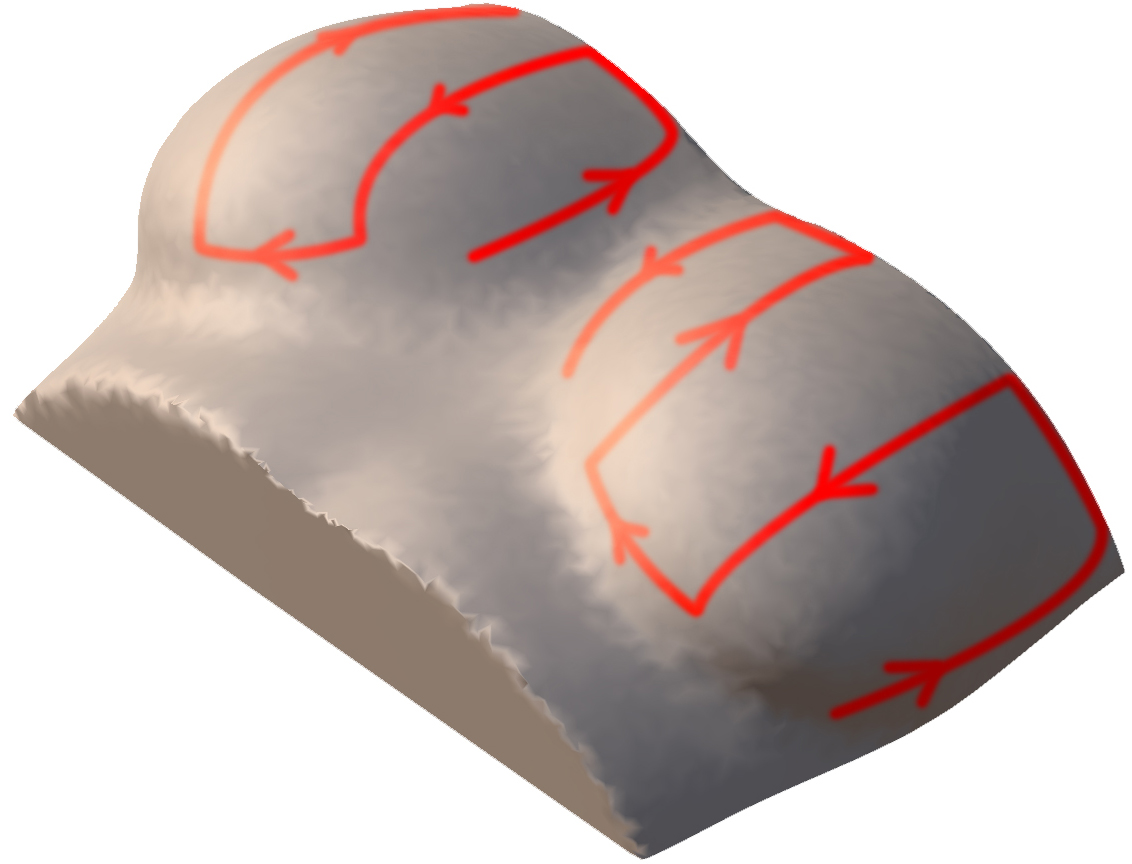
\includegraphics[width=0.75\textwidth]{figurer/d/probebevagelse}
    \caption{Det specifikke bevægelsesmønster ved scanning}
    \label{Probensbevagelse}
\end{figure}

Lars Bolvig tilføjede også, at Automatisk Ultralydsscanner skal kunne betjenes af radiografer. Automatisk Ultralydsscanner skal fungere ved, at radiografen tager videoklippene fra ultralydsscanningen og sender dem til radiologen, som vurderer videoklippene og ud fra det, bestemmer videre behandlingsforløb.

Se bilag \ref{Telefoninterview} Interview med radiolog Lars Bolvig, for hele interviewet. 

\section{Økonomiske konsekvenser ved udvidelse af screeningsprogrammet} 
Formålet med analysen er at belyse det økonomiske perspektiv, hvis mammografiscreeningsprogrammet bliver udvidet til at inkludere ultralydsscanninger. Den økonomiske analyse er udført ved at lave et overslag over forskellen på udgifterne, hvis en radiolog skulle udføre ultralydsscanningerne, versus indførsel og implementering af Automatisk Ultralydsscanner, hvor en radiograf udfører ultralydsscanningerne. 

Analysen tager udgangspunkt i en breakeven analyse.  Efter interview med radiolog Lars Bolvig, blev det sandsynliggjort, at screeingsprogrammet kan udvides med ultralydsscanninger, hvor radiografer betjenet Automatisk Ultralydsscanner. Det vil være samme procedure, som ved mammografi, hvor radiologen gennemser scanningen. 

Analysen tager udgangspunkt i en breakeven analyse.  Efter interview med radiolog Lars Bolvig, blev det sandsynliggjort, at screeingsprogrammet kan udvides med ultralydsscanninger, hvor radiografer betjenet Automatisk Ultralydsscanner. Det vil være samme procedure, som ved mammografi, hvor radiologen gennemser scanningen. 

Ifølge Lars Bolvig, bruger radiologer meget tid på at transportere sig til og fra scanningsstedet, f.eks. fra Aarhus til Holstebro, når der skal scannes på patienter.  Transporttid er derfor en vigtig variabel i breakeven analysen. Breakeven-analysen tager udgangspunkt i, hvor mange ressourcer der kan flyttes fra en radiolog til en radiograf, ift. omkostningen relateret til implementeringen af Automatisk Ultralydsscanner, hvis screeningsprogrammet udvides.  

Det er antaget, at en radiologs gennemsnitlig løn er omkring 369 kr./timen, mens en radiografs gennemsnitlige løn er omkring 173 kr./timen \cite{Lon}. De samlede omkostninger for anskaffelse af udstyret til opsætning af Automatisk Ultralydsscanner er fundet ved indsamling af priser fra forskellige hjemmesider. De samlede faste omkostninger for fuld implementering inkluderer engangsudgifter for opsætning og oplæring af radiografer i anvendelse af Automatisk Ultralydsscanner, hvor det er antaget, at der oplæres fire radiologer på 4 timer af én underviser.  Den samlede pris for Automatisk Ultralydsscanner ligger omkring 219.305,64 kroner, og de samlede udgifter kan ses i Tabel \ref{FasteOmkostninger}.  Se bilag \ref{Okonomi} Økonomisk analyse for alle beregninger. 

\begin{table}[htb]
\centering
\begin{tabular}{ | l | l | p{1\textwidth} | }
\hline
\textbf{Beskrivelse af udgift} & \textbf{DKK} \\\hline
Engangsudgifter til afskrivning & 201.668,00 \\\hline
Opsætning & 10.759,00 \\\hline
Oplæring af radiografer & 6.768,00 \\\hline
I alt & 219.305,64 \\\hline
\end{tabular}
\caption{Samlede udgifter for Automatisk Ultralydsscanner}
\label{FasteOmkostninger}
\end{table}

Der er for begge scenarier blevet beregnet en pris for én ultralydsscanning. Der er lavet antagelser af tidsforbruget ud fra interview med radiolog Lars Bolvig og radiograf Tine Bisgaard. Prisen for én scanning med Automatisk Ultralydsscanner er udregnet ved at antage, at det er en radiograf, der foretager forberedelse, 3D scanning og selve ultralydsscanningen, hvorefter en radiolog vil bruge omkring 10 minutter på at tjekke scanningen igennem for at se, om patienten skal til en yderligere scanning. Prisen for dette er beregnet til 110,64 kroner. Se bilag \ref{Okonomi} Økonomisk analyse for tidsetimeringer og yderligere beregninger. 

Prisen for én ultralydsscanning ved scenariet, hvor en radiolog foretager ultralydsscaningen, er udregnet ved at antage, at det er en radiolog, der foretager både forberedelse, ultralydsscreening og har en transporttid på at komme frem og tilbage til scanningsstedet. Hvis transport for radiologen er under fire minutter, er scenariet med Automatisk Ultralydsscanner dyrest. Automatisk Ultralydsscanner er derimod billigere pr. scanning, hvis transporttid er over 4 minutter. Tabel \ref{Breakeven} beskriver transportminutter, prisen for én ultralydsscanning udført af radiolog ed den transporttid, og antal scanninger udført, før Automatisk Ultralydsscanner er betalt hjem. Se bilag \ref{Okonomi} Økonomisk analyse for tidsetimeringer og yderligere beregninger. 

\begin{table}[H]
\centering
\begin{tabular}{ | c | c | c | p{0.49\textwidth} | }
\hline
\textbf{Transporttid (min)} & \textbf{Pris per scanning (DKK)} & \textbf{Antal scanninger} \\\hline
5 & 116,89 & 35.052,51 \\\hline
8 & 135,34 & 8.873,09\\\hline
10 & 147,64 & 5.923,66\\\hline
15 & 178,39 & 3.235,19 \\\hline
20 & 209,14 & 2.225,25\\\hline
30 & 270,64 & 1.369,94\\\hline
45 & 362,89 & 868,95 \\\hline
60 & 455,14 & 636,26 \\\hline
\end{tabular}
\caption{Breakeven analyse for antal transportminutter}
\label{Breakeven}
\end{table}

Analysen er et overslag og ikke en nøje udført business case, da alle udregningerne er et skøn. Analysen ville fremstå bedre, hvis der havde medvirket flere radiologer til estimering af tider på ultralydsscanninger. Det er generelt forsøgt at prissætte udgifterne forbundet med indførslen af Automatisk Ultralydsscanner relativt højt for at undgå for mange uforudsete omkostninger. Hvis et hospital vil købe udstyret, vil priserne for opsætning måske være lavere, hvis man laver en indkøbsaftale. Beregningerne har ikke taget højde for, at radiologen udfører flere ultralydsscanninger for en transporttid. Transporttid må derfor ses som et gennemsnit pr. patient.

Der bliver i Danmark udført omkring 270.000 mammografiundersøgelser om året, som en del af screeningsprogrammet \cite{esundhed}. Det betyder, at Automatisk Ultralydsscanner med en pris på 110,64 kroner pr. ultralydsscanning vil øge udgifterne til screeningsprogrammet med omkring 30 mio. kroner årligt, men med yderligere omkostninger til indkøb og vedligeholdelse af Automatisk Ultralydsscanner. 

\subsection{Litteratursøgning om screeninger}
Til at belyse konsekvenserne ved at udvide screeningsprogrammet med ultralyd er der søgt nationale og internationale litteratur om screeninger. 

Argumenter for screeninger er, at behandling af brystkræft på et tidligt stadie kan redde 6 ud af 1.000 kvinder fra at dø \cite{Argumenter}. Et japansk randomized controlled trial (RCT) viste, at der ved kombinationen af ultralyds- og røntgenundersøgelser, blev fundet flere stadie 0 og I kræft i interventionsgruppen, både ultralyds- og røntgenscanninger, mens der ved stadie II ikke var signifikant forskel \cite{Japan}. Det amerikanske Cancer Society har estimeret, at den relative overlevelsesprocent ved stadie 0 og I er tæt på 100\%, en overlevelsesprocent på 93\% ved stadie II, mens stadie III har en på 72\% og stadie IV har en overlevelsesprocent på 22\% \cite{CancerSociety}. Dette taler for at indføre en ultralydsundersøgelser til screeningsprogrammet. 

Argumenterne imod er, at 13 ud af 1.000 kvinder vil blive udsat for overdiagnosticering, hvor patienter unødvendigt overbehandles, og at screeninger kan give falsk tryghed for patienter \cite{Argumenter}. Det japanske RCT studie fandt, at der var en højere rate af falsk-positive tilfælde ved at anvende ultralyd sammen med mammografi \cite{Japan}. Et uafhængigt panel sammensat af Department of Epidemiology and Public Health, UK, undersøgte 11 RCT’er. Panelet estimerede, at ved screening for brystkræft af 10.000 50-årige kvinder, vil 43 brystkræftsrelaterede dødsfald blive forhindret, mens 129 vil blive overdiagnosticeret \cite{Panel}. Et Cochrane review undersøgte RCT’s, der sammenlignede to grupper, hvoraf den ene screenes for brystkræft. Reviewet konkluderede, at screening reducerer brystkræft med 15\%, mens 30\% overdiagnosticeres og får behandling uden grund \cite{Gotzche}. Et BMC Cancer review undersøgte konsekvenserne af at lave en ultralydsscanning af brystet, efter en røntgenundersøgelse med et negativt resultat. Studiet fandt begrænset evidens for, at ultralyd er en fordel. Tre gange så mange kvinder fik lavet en biopsi ved ultralydsscanninger, hvor den positive prædiktive værdi gennemsnitlig er 10,3 \%. Det betyder flere falsk-positive prøver ved biopsier, hvor den positive prædiktive værdi gennemsnitlig er 38\% ved mammografi \cite{DenseBreast}. 

Som pejlemærke til omkostningseffektiviteten kan man benytte kvalitets justerede leveår (QALY) til at beskrive, hvor rentabel en behandling er. I Danmark er der ikke en officiel grænse for, hvor meget én QALY bør koste, men Sundhedsstyrelsen (SST) har beskrevet: ” at man generelt anser behandlinger, der koster mindre end 160.000 kr. pr. QALY for at være omkostningseffektive, mens behandlinger der koster mere end 800.000 kr. pr. QALY anses for ikke at være omkostningseffektive” \cite{QALY}. Et spansk studie undersøgte inkrementelle omkostninger ved henholdsvis ingen, årliger og biennale scanninger. Studiet viste, at gå fra ingen til scanninger hver andet år svarer til 4,469 € per QALY \cite{SpanskStudie}, 33.241,76 danske kroner, hvilket taler for screening efter SST's beskrivelse. National Health Service konkluderede i et RCT, at screeninger var forbundet med en ekstra omkostning på 45.5 mio. pund i det engelske sundhedsvæsen, svarende til 20.800 £ per vunden QALY \cite{NHS}. Dette svarer i danske kroner til 183.335 pr. vunden QALY.  

Støstedelen af litteraturen konkluderer, at mere forskning er nødvendig på området. Det kan derfor være svært at lave en endelig konklusion på, hvorvidt en udvidelse af screeningsforløbet vil være en god idé. Fordelen er, at man ved en kombination af ultralyd og røntgen kan man opdage tidligere stadie af kræft, og at overlevelsesprocenten er højere. Ulemperne er, at der sker overdiagnosticering ved screening, og patienter derfor behandles uden grund, og derfor vil en tilføjelse af ultralydsscanninger til screeningsprogrammet sandsynligvis ikke være omkostningseffektivt. Se bilag \ref{Okonomi} Økonomisk og omkostningseffektiv analyse, for hele analysen. 
